\section{Lựa chọn mô hình và kiến trúc}

\subsection{Tổng quan các mô hình sử dụng}
Nhóm thực nghiệm tổng cộng \textbf{7 mô hình}, bao gồm 6 mô hình học máy truyền thống và 1 mô hình Deep Learning (PhoBERT), được tóm tắt trong Bảng~\ref{tab:model_overview}.

\begin{table}[H]
\centering
\caption{Tổng quan các mô hình thực nghiệm}
\label{tab:model_overview}
\begin{tabular}{|c|l|l|l|}
\hline
\textbf{\#} & \textbf{Mô hình} & \textbf{Loại} & \textbf{Input Feature} \\
\hline
1 & Logistic Regression & Tuyến tính & TF-IDF \\
2 & Multinomial Naive Bayes & Xác suất & Bag-of-Words \\
3 & Linear SVC & Tuyến tính (SVM) & TF-IDF \\
4 & Random Forest & Ensemble (Bagging) & TF-IDF + SVD \\
5 & SGD Classifier & Tuyến tính (SGD) & TF-IDF \\
6 & Voting Ensemble & Meta-ensemble & TF-IDF \\
7 & PhoBERT-base-v2 & Deep Learning (Transformer) & Tokenized text \\
\hline
\end{tabular}
\end{table}

\subsection{Lý do lựa chọn từng mô hình}

\textbf{Logistic Regression} \parencite{cox1958lr} được chọn làm baseline mạnh nhờ tính diễn giải cao, hội tụ nhanh trên dữ liệu TF-IDF \parencite{salton1988tfidf} sparse, và khả năng regularization linh hoạt qua tham số $C$.

\textbf{Multinomial Naive Bayes} \parencite{mccallum1998nb} là mô hình xác suất cổ điển cho bài toán phân loại văn bản, dựa trên định lý Bayes với giả định các đặc trưng độc lập có điều kiện. Mô hình này yêu cầu input không âm nên sử dụng Bag-of-Words thay vì TF-IDF.

\textbf{Linear SVC} (Support Vector Classifier) \parencite{cortes1995svm} tìm siêu phẳng phân tách tối ưu trong không gian đặc trưng, thường đạt hiệu suất cao cho bài toán phân loại văn bản với TF-IDF.

\textbf{Random Forest} \parencite{breiman2001rf} là ensemble của nhiều cây quyết định, mỗi cây huấn luyện trên tập con ngẫu nhiên. Do ma trận TF-IDF 10{,}000 chiều quá lớn cho Random Forest, nhóm áp dụng \textbf{TruncatedSVD} giảm xuống 300 chiều trước khi huấn luyện.

\textbf{SGD Classifier} \parencite{bottou2010sgd} sử dụng Stochastic Gradient Descent để huấn luyện mô hình tuyến tính, cho phép ghi nhận loss và accuracy theo từng epoch --- đáp ứng yêu cầu vẽ biểu đồ quá trình học (learning curves).

\textbf{Voting Ensemble} \parencite{dietterich2000ensemble} kết hợp dự đoán của Logistic Regression, Linear SVC (calibrated) và SGD Classifier bằng phương pháp \textit{soft voting} (trung bình xác suất), nhằm tận dụng ưu điểm của từng mô hình thành viên.

\textbf{PhoBERT-base-v2} \parencite{phobert2020} là mô hình ngôn ngữ pre-trained dành riêng cho tiếng Việt, dựa trên kiến trúc RoBERTa \parencite{liu2019roberta}. PhoBERT được fine-tune cho bài toán phân loại 3 lớp, kỳ vọng nắm bắt ngữ nghĩa sâu hơn so với TF-IDF.

\subsection{Sơ đồ pipeline tổng quát}

Hình~\ref{fig:arch_pipeline} mô tả luồng xử lý dữ liệu từ văn bản thô đến nhãn dự đoán cho cả hai nhánh: mô hình truyền thống (TF-IDF) và Deep Learning (PhoBERT).

\begin{figure}[H]
\centering
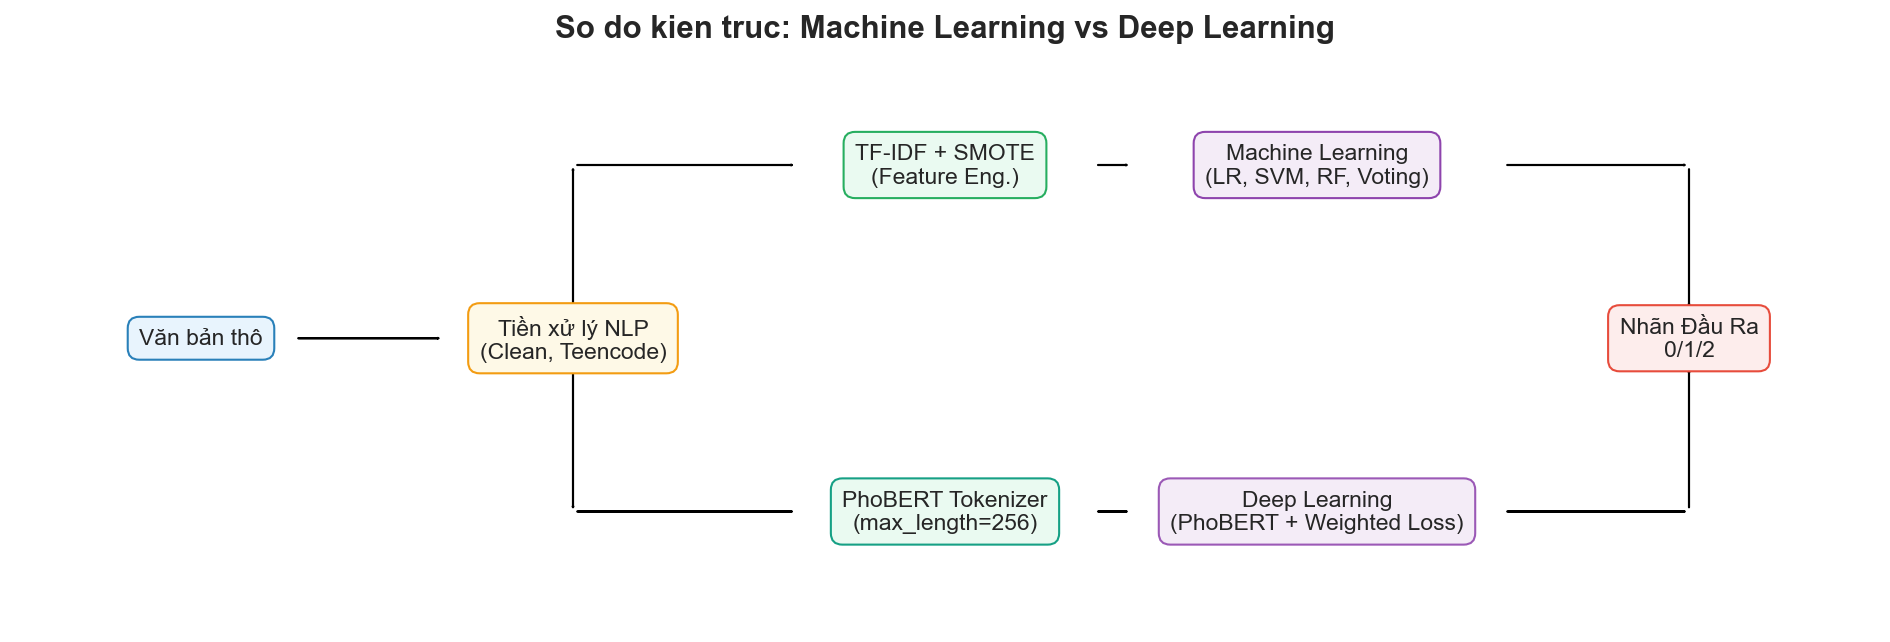
\includegraphics[width=0.95\textwidth]{figures/arch_pipeline.png}
\caption{Sơ đồ pipeline phân loại bình luận tiêu cực tiếng Việt}
\label{fig:arch_pipeline}
\end{figure}

\subsection{Kiến trúc chi tiết - PhoBERT (Deep Learning)}

\textbf{Kiến trúc:} PhoBERT-base-v2 dựa trên RoBERTa gồm 12 lớp Transformer encoder \parencite{vaswani2017transformer}, mỗi lớp có 12 attention heads, kích thước hidden state 768. Tổng cộng khoảng \textbf{135 triệu tham số} (bao gồm embedding + encoder + classification head).

\textbf{Classification Head:} Đầu ra CLS token được đưa qua lớp Dense (768 $\rightarrow$ 768, hàm kích hoạt Tanh) rồi qua lớp phân loại tuyến tính (768 $\rightarrow$ 3, hàm kích hoạt Softmax qua Cross-Entropy Loss).

\textbf{Tokenization:} Sử dụng BPE tokenizer của PhoBERT với \texttt{max\_length=256}, \texttt{padding="max\_length"}, \texttt{truncation=True}.

%---------------------------------------------------
\section{Cấu hình huấn luyện}

\subsection{Xử lý mất cân bằng dữ liệu}

Dữ liệu mất cân bằng nghiêm trọng (CLEAN: 82\%, OFFENSIVE: 7\%, HATE: 11\%), nhóm áp dụng hai chiến lược:
\begin{itemize}
    \item \textbf{SMOTE} \parencite{chawla2002smote} (Synthetic Minority Over-sampling Technique): tổng hợp mẫu nhân tạo cho lớp thiểu số trên không gian TF-IDF/BoW, nâng tập train từ 22{,}510 lên 55{,}419 mẫu (cân bằng 3 lớp).
    \item \textbf{class\_weight='balanced'}: thử nghiệm qua GridSearchCV cho LR, SVM - tự điều chỉnh trọng số tỷ lệ nghịch với tần suất lớp.
    \item \textbf{Weighted Cross-Entropy} (PhoBERT): tính class weights bằng \texttt{compute\_class\_weight('balanced')} và truyền vào \texttt{nn.CrossEntropyLoss(weight=...)}.
\end{itemize}

\subsection{Hàm mất mát}

Bảng~\ref{tab:loss_functions} tóm tắt hàm mất mát của từng mô hình.

\begin{table}[H]
\centering
\caption{Hàm mất mát theo từng mô hình}
\label{tab:loss_functions}
\begin{tabular}{|l|l|l|}
\hline
\textbf{Mô hình} & \textbf{Hàm mất mát} & \textbf{Lý do} \\
\hline
Logistic Regression & Cross-Entropy (Log Loss) & Chuẩn cho phân loại đa lớp \\
Multinomial NB & Negative Log-Likelihood & Ước lượng MLE + Laplace smoothing \\
Linear SVC & Squared Hinge Loss & Tối ưu margin, hiệu quả với SVM \\
Random Forest & Gini Impurity & Tiêu chuẩn phân chia node \\
SGD Classifier & Log Loss (Cross-Entropy) & Tương đương LR, hỗ trợ partial\_fit \\
Voting Ensemble & - & Kết hợp xác suất từ các mô hình con \\
PhoBERT & Weighted Cross-Entropy & Có trọng số lớp để xử lý imbalance \\
\hline
\end{tabular}
\end{table}

\subsection{Thuật toán tối ưu}

\begin{itemize}
    \item \textbf{Logistic Regression}: L-BFGS (Limited-memory BFGS) - hiệu quả cho multiclass, \texttt{max\_iter=1000}.
    \item \textbf{Linear SVC}: Liblinear (coordinate descent) - tối ưu cho bài toán tuyến tính trên sparse matrix.
    \item \textbf{SGD Classifier}: Stochastic Gradient Descent với \texttt{learning\_rate='optimal'} (tự điều chỉnh), \texttt{penalty='l2'}, 20 epochs.
    \item \textbf{Random Forest / NB}: Không sử dụng gradient descent - RF dùng greedy splitting, NB dùng MLE.
    \item \textbf{PhoBERT}: AdamW optimizer \parencite{loshchilov2019adamw}, \texttt{learning\_rate=2e-5}, \texttt{weight\_decay=0.01}, 3 epochs, \texttt{fp16=True} (mixed precision).
\end{itemize}

\subsection{Siêu tham số và phương pháp tinh chỉnh}

Tất cả mô hình truyền thống được tối ưu bằng \textbf{GridSearchCV} \parencite{sklearn2011} với \texttt{StratifiedKFold(n\_splits=3)}, \texttt{scoring='f1\_weighted'}, \texttt{n\_jobs=-1}. Bảng~\ref{tab:hyperparams} liệt kê siêu tham số và không gian tìm kiếm.

\begin{table}[H]
\centering
\caption{Siêu tham số và kết quả GridSearchCV}
\label{tab:hyperparams}
\begin{tabular}{|l|l|l|}
\hline
\textbf{Mô hình} & \textbf{Không gian tìm kiếm} & \textbf{Tham số tối ưu} \\
\hline
Logistic Regression & C: [0.01, 0.1, 1, 10] & C=10, class\_weight=None \\
 & class\_weight: [None, balanced] & \\
\hline
Multinomial NB & alpha: [0.1, 0.5, 1.0, 2.0] & alpha=0.1 \\
\hline
Linear SVC & C: [0.1, 1, 5, 10] & C=10, class\_weight=balanced \\
 & class\_weight: [None, balanced] & \\
\hline
Random Forest & n\_estimators: [100, 200] & n\_estimators=200 \\
 & max\_depth: [10, 30, 50, None] & max\_depth=None \\
 & class\_weight: [balanced] & class\_weight=balanced \\
\hline
SGD Classifier & alpha: [1e-4, 1e-3] & alpha=1e-4 \\
 & class\_weight: [None, balanced] & class\_weight=None \\
\hline
PhoBERT & batch\_size: 16, epochs: 3 & - (thử nghiệm thủ công) \\
 & lr: 2e-5, max\_length: 256 & \\
\hline
\end{tabular}
\end{table}
